% --------------------------------------------------------------
% gabarito feito + 35 exercícios convertidos para múltipla escolha
% --------------------------------------------------------------
 
\documentclass[12pt]{article}\documentclass[brazilian,12pt,a4paper,final]{article}
\usepackage[brazil]{babel}
\usepackage[utf8]{inputenc}
\usepackage{graphicx}
\usepackage{color}
\usepackage{setspace}
\usepackage{ulem} 
\usepackage[margin=1in]{geometry} 
\usepackage{amsmath,amsthm,amssymb}
\usepackage{enumitem}
\newcommand{\N}{\mathbb{N}}
\newcommand{\Z}{\mathbb{Z}}
 
\newenvironment{theorem}[2][Theorem]{\begin{trivlist}
\item[\hskip \labelsep {\bfseries #1}\hskip \labelsep {\bfseries #2.}]}{\end{trivlist}}
\newenvironment{lemma}[2][Lemma]{\begin{trivlist}
\item[\hskip \labelsep {\bfseries #1}\hskip \labelsep {\bfseries #2.}]}{\end{trivlist}}
\newenvironment{exercise}[2][Exercise]{\begin{trivlist}
\item[\hskip \labelsep {\bfseries #1}\hskip \labelsep {\bfseries #2.}]}{\end{trivlist}}
\newenvironment{reflection}[2][Reflection]{\begin{trivlist}
\item[\hskip \labelsep {\bfseries #1}\hskip \labelsep {\bfseries #2.}]}{\end{trivlist}}
\newenvironment{proposition}[2][Proposition]{\begin{trivlist}
\item[\hskip \labelsep {\bfseries #1}\hskip \labelsep {\bfseries #2.}]}{\end{trivlist}}
\newenvironment{corollary}[2][Corollary]{\begin{trivlist}
\item[\hskip \labelsep {\bfseries #1}\hskip \labelsep {\bfseries #2.}]}{\end{trivlist}}
 
\begin{document}
 
 
\title{Exercícios}%replace X with the appropriate number
\author{\\ %replace with your name
MAT02219 - Probabilidade e estatística} %if necessary, replace with your course title
 
\maketitle
 \begin{enumerate} 
 %começo do capítulo 4

\section*{CAPÍTULO 4 media mediana desvio padrão}

\section{CAPÍTULO 4}

 \item (área 1 - média) \begin{enumerate}[label=(\Roman*)] \item Os números 3 e 5 são marcados com cruzes na linha horizontal abaixo. Encontre
a média desses dois números e marque-a com uma seta.

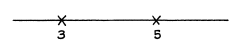
\includegraphics{Figuras/Capítulo 4/4A1a.png}
\item Repita (I) para a lista de números 3, 5, 5.

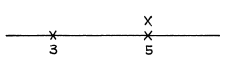
\includegraphics{Figuras/Capítulo 4/4A1b.png}
\item Dois números são mostrados abaixo por cruzamentos em um eixo horizontal. Desenhe uma flecha
apontando para sua média.

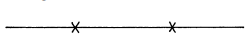
\includegraphics{Figuras/Capítulo 4/4A1c.png}
\end{enumerate}
Os locais onde devem ser marcadas as setas são, respectivamente:
\begin{enumerate}[label=(\alph*)]
\item No meio dos pontos 3 e 5, no meio dos pontos 3 e 5, no meio dos pontos. 

\item Entre os pontos 3 e 5 mas mais perto do 3, entre os pontos 3 e 5 mas mais perto do 5, no meio dos pontos.

\item No meio dos pontos 3 e 5, entre os pontos 3 e 5 mas mais perto do 5, no meio dos pontos.

\item Antes do ponto 3, depois do ponto 5, antes do primeiro ponto.

\item No meio dos pontos 3 e 5, no meio dos pontos 3 e 5, depois do segundo ponto.

\end{enumerate}

\textbf{Respostas:(c)(I) 4 (II) 4,3 (III) No meio dos 2 pontos.}


\item (área 1 - média) Uma lista possui 10 entradas. Cada entrada pode ser 1, 2 ou 3. Qual deve ser a lista se a
média é 1? E se a média for 3? A média pode ser 4?

\begin{enumerate}
    \item Há uma combinação de listas que satisfazem média 1, há uma combinação de listas que satisfazem média 3, a média pode ser 4.
    \item Há uma combinação de listas que satisfazem média 1, há uma combinação de listas que satisfazem média 3, a média não pode ser 4.
    \item A única lista que satisfaz média 1 consiste em dez 1's, a única lista que satisfaz média 3 consiste em dez 3's, a média pode ser 4.
    \item A única lista que satisfaz média 1 consiste em dez 1's, a única lista que satisfaz média 3 consiste em dez 3's, a média não pode ser 4.
    \item A única lista que satisfaz média 1 consiste em dez 1's, há uma combinação de listas que satisfazem média 3, a média não pode ser 4.
    
\end{enumerate}

\textbf{Resposta:(d) Se a média for 1, a lista consiste em dez 1's. Se a média for 3, a lista consiste em dez 3's. A média não pode ser 4: precisa entre 1 e 3.
}

\item (área 1 - média) Qual das três listas a seguir tem uma média maior? Ou elas tem a mesma média? Tente responder sem fazer nenhuma conta.
(i)10, 7, 8, 3, 5, 9 \hspace{0,8cm} (ii) 10, 7, 8, 3, 5, 9, 11 \hspace{0,8cm} (iii)10, 7, 8, 3, 5, 9, 11, 11
Nas alternativas, média da lista (i) = M(i), e assim sucessivamente.
\begin{enumerate}
    \item M(i) = M(ii) = M(iii)
    \item M(i) > M(ii) > M(iii)
    \item M(i) < M(ii) > M(iii)
    \item M(i) < M(ii) = M(iii)
    \item M(i) < M(ii) < M(iii)
\end{enumerate}


\textbf{Resposta:(e)A média de (ii) é maior que a média de (i), pois (ii) contém (i) + o número 11, e a média de (iii) é maior que a média de (ii), pois (iii) contém (ii) + outro número superior a M(ii).} 

\item (área 1 - média para amostras de tamanhos diferentes) \begin{enumerate}[label=(\Roman*)] 
\item Dez pessoas em uma sala têm uma altura média de 1,68 metro. Uma 11ª pessoa,
quem tem 1,96m de altura, entra na sala. Encontre a altura média de todas as 11 pessoas.
\item Vinte e uma pessoas em uma sala têm uma altura média de 1,68 metro. Uma 22ª pessoa,
quem tem 1,96m de altura, entra na sala. Encontre a altura média de todas as 22 pessoas e compare com o item anterior.
\end{enumerate}
As respostas para os dois itens são:
\begin{enumerate}
    \item (I) 1,705m; (II) 1,69m. Conforme o número de pessoas na sala aumenta, cada pessoa adicional tem um efeito menor na média.
    \item (I) 1,73m; (II) 1,715m. Conforme o número de pessoas na sala aumenta, cada pessoa adicional tem um efeito menor na média.
    \item (I) 1,68m; (II)1,715m. Conforme o número de pessoas na sala aumenta, cada pessoa adicional tem um efeito maior na média.
    \item (I) 1,705m; (II) 1,69m. Conforme o número de pessoas na sala aumenta, cada pessoa adicional tem um efeito maior na média.
    \item (I) 1,77m; (II) 1,64m. Conforme o número de pessoas na sala aumenta, cada pessoa adicional tem um efeito menor na média.
\end{enumerate}
\textbf{Resposta:(a)(I)(10x1,68+1,96)/11=1,705m ou pode ser pensado dessa forma: A nova pessoa é 0,28m mais alta do que a média antiga. Então ela adiciona 0,28m/11 à média.
 (II) 1,69m - Conforme o número de pessoas na sala aumenta, cada pessoa adicional tem um efeito menor na média.}
 

\item (área 1 - média) Vinte e uma pessoas em uma sala têm uma altura média de 1,68 metro. Uma 22ª pessoa, entra na sala. Qual deve ser a sua altura para que a média da sala aumente em 2 cm?
\begin{enumerate}[label=(\alph*)]
    \item 1,70m
    \item 1,86m
    \item 1,94m
    \item 2,02m
    \item 2,12m
\end{enumerate}

\textbf{Resposta:1,68+0,02x22= 2,12m }

\item(área 1 - gráficos - explicação para um padrão) A pressão arterial diastólica é considerada um melhor indicador de problema cardíaco do que a pressão sistólica. A figura abaixo mostra a pressão arterial diastólica média específica da idade para os homens com 20 anos ou mais de idade em HANES5 (2003-04) .6

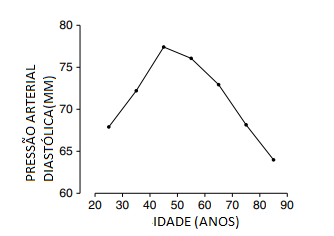
\includegraphics{Figuras/Capítulo 4/4A8.png}

Quanto ao padrão do gráfico, faz sentido concluir que:
\begin{enumerate}
    \item À medida que os homens envelhecem, a pressão arterial diastólica aumenta até os 45 anos, e depois diminui.
    \item À medida que os homens envelhecem, a pressão arterial diastólica diminui até os 45 anos, e depois aumenta.
    \item Homens com pressão arterial diastólica mais baixa provavelmente morrerão mais cedo, e por isso não serão
representado no gráfico. Além disso, homens com pressão arterial mais baixa são mais propensos ao uso de medicamentos que aumentam a pressão arterial. 
    \item Homens com pressão arterial diastólica mais alta provavelmente morrerão mais cedo, e por isso não serão
representado no gráfico. Além disso, homens com pressão arterial mais alta são mais propensos ao uso de medicamentos que reduzem a pressão arterial. 
    \item Nenhuma das alternativas anteriores.

\end{enumerate}

\textbf{Resposta:(d)Os dados são transversais, não longitudinais. Homens com pressão arterial diastólica mais alta provavelmente morrerão mais cedo, e por isso não serão
representados no gráfico. Além disso, homens com pressão arterial mais alta são mais
propensos ao uso de medicamentos que reduzem a pressão arterial.}


\item (área 1 - explicação para uma variação da média) Os ganhos médios por hora são calculados todos os meses pelo Bureau of Labor Statistics usando dados da folha de pagamento de estabelecimentos comerciais. A Repartição calcula os
salários totais pagos e divide pelo total de horas
trabalhadas. Durante as recessões, os ganhos médios por hora geralmente aumentam. Quando a recessão termina, os ganhos médios por hora geralmente começam a cair. Como isso pode acontecer?

\begin{enumerate}
    \item Durante as recessões, as empresas tendem a demitir os trabalhadores mais antigos, que
também são os que recebem os salários mais altos. Isso aumenta o salário médio daqueles que permanecem na folha de pagamento.
Quando a recessão termina, esses trabalhadores bem remunerados são recontratados.
    \item Durante as recessões, as empresas tendem a demitir os trabalhadores mais novos, que
também são os que recebem os salários mais baixos. Isso aumenta o salário médio daqueles que permanecem na folha de pagamento.
Quando a recessão termina, esses trabalhadores mal remunerados são recontratados.
    \item Durante as recessões, as empresas tendem a expandir, e com isso, contratam novos funcionários, o que aumenta o salário médio.
    Após as recessões, esses funcionários são demitidos, o que diminui o salário médio.
    \item Durante as recessões, as empresas aumentam o salário dos seus funcionários, mas apenas provisoriamente, pois assim que a recessão acaba, os salários são reduzidos novamente.
    \item Nenhuma das alternativas anteriores.
\end{enumerate}

\textbf{Resposta:(b) Durante as recessões, as empresas tendem a demitir os trabalhadores mais novos, que
também são os que recebem os salários mais baixos. Isso aumenta o salário médio daqueles que permanecem na folha de pagamento.
Quando a recessão termina, esses trabalhadores mal remunerados são recontratados.}


\item (área 1 - média em histograma) Abaixo estão esboços de histogramas para três listas. Respectivamente, para cada lista, a
média é em torno de: Opções: 25, 40, 50, 60, 75.

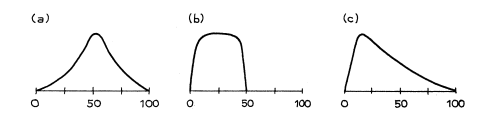
\includegraphics{Figuras/Capítulo 4/4B1.png}

\begin{enumerate}
    \item 75, 50, 60
    \item 40, 60, 75.
    \item 50, 25, 75.
    \item 25, 20, 80.
    \item 50, 25, 40.
\end{enumerate}

\textbf{Resposta: (e)Listas: (a) 50 (b) 25 (c) 40}

\item (área 1 - mediana e média em histograma)Respectivamente, para cada um dos  histogramas a seguir, a mediana é igual à média? Se não é, está posicionada à esquerda ou à direita da média?

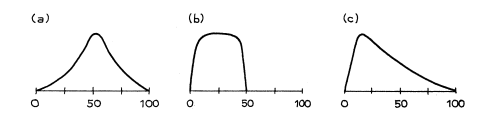
\includegraphics{Figuras/Capítulo 4/4B1.png}

\begin{enumerate}
    \item mediana = média; mediana à direita da média; mediana=média.
    \item mediana para a direita da média; mediana=média; mediana à  esquerda da média.
    \item mediana = média; mediana=média; mediana à esquerda da média.
    \item mediana à esquerda da média; mediana à esquerda da média; mediana=média.
    \item mediana = média; mediana=média; mediana à direita da média.
\end{enumerate}

\textbf{Resposta:(e)Histogramas: (a) mediana = média (b) mediana = média
(c) mediana está para a esquerda da média.}

\item (área 1 - mediana e média em histograma) Em um estudo do Serviço Público de Saúde, um histograma foi plotado mostrando o número
cigarros por dia fumados por cada cobaia (fumantes atuais), como mostrado
abaixo. A densidade é marcada entre parênteses. Os intervalos das classes incluem o ponto final à direita, não a esquerda.

 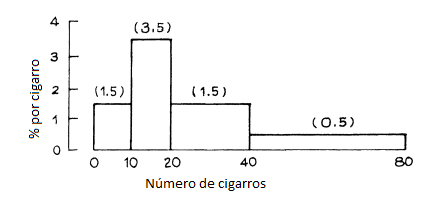
\includegraphics{Figuras/Capítulo 3/3C4.png}
 
A mediana e a média, para este histograma, estão em torno de:
\begin{enumerate}
    \item Mediana: 10, Média: 20.
    \item Mediana: 30, Média: 25.
    \item Mediana: 20, Média: 25.
    \item Mediana: 20, Média: 15.
    \item Mediana: 40, Média: 30.
\end{enumerate}Opções: 10, 20, 30, 40.

\textbf{Reposta:(d)A mediana é 20, e a média deve ser maior do que 20, então entre as duas opções, 25 é a única que faz  sentido. (A resposta exata é 27.)}

\item (área 1 - média e mediana, generalizações) Para estudantes registrados em universidades no Brasil, quanto a relação entre a idade média e a idade mediana, uma conclusão razoável é a de que:
\begin{enumerate}
    \item No geral, Idade média $>$ Idade mediana.
    \item Em cada uma das universidades, Idade média $>$ Idade mediana.
    \item No geral, Idade média $<$ Idade mediana.
    \item Em cada uma das universidades, Idade média $<$ Idade mediana
    \item Idade média = Idade mediana.
\end{enumerate}

\textbf{Resposta:(a)A média é maior, pois um grande número de pessoas na faixa dos 20 anos faz com que a mediana seja em torno desse valor,  e pessoas mais velhas aumentam a média, mas não a mediana. Embora essa conclusão seja válida para os dados em geral, não pode ser dito que é válida em cada uma das universidades, por isso (b) não é razoável.)}

\item (área 1 - média) Para cada uma das seguintes listas de números, diga, se a média está em torno de 1, 5 ou 10. (Não é necessário fazer as contas).
\begin{enumerate}[label=(\Roman*)]
\item1,3; 0.9; 1,2; 0.8 
\item13; 9; 12; 8
\item7; 3; 6; 4 
\item7; −3; −6; 4
\end{enumerate}
\begin{enumerate}
    \item (I) 10 (II) 5 (III) 1 (IV) 1
    \item (I) 1 (II) 5 (III) 5 (IV) 5
    \item (I) 1 (II) 10 (III) 5 (IV) 5
    \item (I) 5 (II) 10 (III) 10 (IV) 1
    \item (I) 1 (II) 5 (III) 10 (IV) 5
    
\end{enumerate}

\textbf{Respostas:(c)(I) 1 (II) 10 (III) 5 (IV) 5}

\item (área 1 - média e RMS) Encontre a média e a raiz do valor quadrático médio (RMS) dos números nas listas a seguir.
\begin{enumerate}[label=(\Roman*)]
\item 1, −3, 5, −6, 3.
\item −11, 8, −9, −3, 15.
\end{enumerate}
\begin{enumerate}
    \item (I) média = 0, RMS = 4. (II) média = 0, RMS = 5.
    \item (I) média = -1, RMS = 3. (II) média = 0, RMS = 10.
    \item (I) média = 1, RMS = -3. (II) média = 2, RMS = 10.
    \item (I) média = 0, RMS = 5. (II) média = -1, RMS = 10.
    \item (I) média = 0, RMS = 4. (II) média = 0, RMS = 10.
    \end{enumerate}
\textbf{Resposta:(e)  (I) média = 0, RMS = 4
(II) média = 0, RMS = 10.
No total, os números na lista (b) são maiores em tamanho.
}

\item (área 1 - RMS) Adivinhe se a raiz do valor quadrático médio de cada uma das seguintes listas de números é de cerca de
1, 10 ou 20. (Não é necessário fazer as contas).
\begin{enumerate}[label=(\Roman*)]
\item 1, 5, −7, 8, −10, 9, −6, 5, 12, −17
\item 22, −18, −33, 7, 31, −12, 1, 24, −6, −16
\item 1, 2, 0, 0, −1, 0, 0, −3, 0, 1
\end{enumerate}
\begin{enumerate}
    \item (I) 1 (II) 20 (III) 1
    \item (I) 10 (II) 20 (III) 1
    \item (I) 10 (II) 1 (III) 20
    \item (I) 20, (II) 20, (III) 10
    \item (I) 10, (II) 1, (III) 20
\end{enumerate}

\textbf{Resposta:(b) (I) 10 (com uma casa decimal, a resposta exata é 9,0).
(II) 20 (com uma casa decimal, a resposta exata é 19,8).
(III) 1 (com uma casa decimal, a resposta exata é 1,3).
A média das listas é 0; a operação da r.m.s, apaga os sinais.}

\item(área 1 - RMS) A raiz do valor quadrático médio das listas
    \begin{enumerate}[label=(\Roman*)]
    \item 7, 7, 7, 7.
    \item 7, −7, 7, −7.
    \end{enumerate}
é, respectivamente:
\begin{enumerate}
    \item 0, 0.
    \item 0, 14.
    \item 7, 7.
    \item 7, -7.
    \item 7, 0.
\end{enumerate}

\textbf{Resposta:(c) Nas duas listas, é 7; todas as entradas têm o mesmo tamanho, 7.}

\item (área 1 - desvio RMS) Cada um dos números 103, 96, 101, 104 é quase 100, mas tem um desvio de alguma quantidade.
Encontre a raiz do valor quadrático médio desses desvios.

\begin{enumerate}
    \item 6,4
    \item 8,3
    \item 5,0
    \item 3,2
    \item 1,8
\end{enumerate}
\textbf{Resposta:(d) 3,2}

\item (área 1 - desvio RMS e média) A lista 103, 96, 101, 104 tem uma média. Cada número da lista tem um desvio em relação à média de algum valor. Encontre a raiz do valor quadrático médio dos desvios.
\begin{enumerate}
    \item 5,5
    \item 3,1
    \item 3,7
    \item 4,2
    \item 1,8
\end{enumerate}


\textbf{Resposta:(b) 3,1}

\item (área 1 - RMS) Um computador está programado para prever as pontuações dos testes, compará-las com as pontuações reais e encontrar
a raiz do valor quadrático médio dos erros de previsão. Olhando para a impressão,
você vê que a raiz do valor quadrático médio dos erros de previsão é 3,6 e os resultados para os dez primeiros alunos
são os seguintes:

Pontuação prevista: 90 90 87 80 42 70 67 60 83 94

\hspace{0,8cm}Pontuação real: 88 70 81 85 63 77 66 49 71 69

A impressão parece razoável ou há algo errado com o computador?
\begin{enumerate}
    \item  Algo está errado com o computador, pois os erros são muito maiores que 3,6; que deveria ser a raíz do valor quadrático médio, 
    \item  A impressão parece razoável, pois os erros são muito menores que 3,6; que deveria ser a raíz do valor quadrático médio.
    \item  Algo está errado com o computador, mas a raiz do valor quadrático médio não é um bom parâmetro de comparação.
    \item A impressão parece razoável, mas a raiz do valor quadrático médio não é um bom parâmetro de comparação.
    \item Não há informações suficientes para responder.
\end{enumerate}

\textbf{Resposta:(a) Os erros são muito maiores que 3,6; que deveria ser a raíz do valor quadrático médio, Algo está errado com o computador}

%set D
\item (área 1 - Desvio padrão) O Serviço Público de Saúde constatou que, para meninos de 11 anos no HANES2, a média
de altura foi de 146 cm e o desvio padrão (DP) foi de 8 cm.
\begin{enumerate}[label=(\Roman*)]
\item Um garoto tinha 170 cm de altura. Ele estava acima da média, por \_\_\_\_\_\_\_ DPs.
\item Outro garoto tinha 148 cm de altura. Ele estava acima da média, por \_\_\_\_\_\_\_ DPs.
\item Um terceiro garoto tinha 1,5 DPs abaixo da altura média. Ele tinha \_\_\_\_\_\_\_\_ cm de altura.
\item Se um garoto estivesse entre 2,25 DPs da estatura média, o mais baixo que ele poderia ser é \_\_\_\_\_\_\_\_ cm e o mais alto seria \_\_\_\_\_\_\_\_ cm.
\end{enumerate}
As respostas que preenchem os espaços em branco são, respectivamente:
\begin{enumerate}
    \item 1; 0,5; 134; 120; 164.
    \item 2; 0,25; 155; 134; 180.
    \item 0,25; 2; 157; 125; 178
    \item 3; 1,25; 152; 164; 178.
    \item 3; 0,25; 134; 128; 164.
\end{enumerate}
Resposta:
(e)
(I) 170 cm está 24 cm acima da média, o DP é de 8 cm; portanto, 24 cm representa 3 DPs.

(II) 2 cm é 0,25 DP.

(III) 1,5 × 8 = 12 cm, o menino tem 146 - 12 = 134 cm de altura.

(IV) menor, 146-18 = 128 cm; mais alto, 146 + 18 = 164 cm

\item (área 1 - média e desvio padrão) O Serviço Público de Saúde constatou que, para meninos de 11 anos no HANES2, a média
de altura foi de 146 cm e o desvio padrão (DP) foi de 8 cm. 

Seguem as alturas de quatro meninos: 150 cm, 130 cm, 165 cm, 140 cm.

Combine as alturas com as descrições.
\begin{enumerate}[label=(\Roman*)]
\item Extraordinariamente baixo \item Aproximadamente na média \item Extraordinariamente  alto
\end{enumerate}
\begin{enumerate}
    \item 150cm - (III); 130cm - (I); 165cm - (II); 140cm - (II).
    \item 150cm - (II); 130cm - (I); 165cm - (III); 140cm - (II).
    \item 150cm - (II); 130cm - (II); 165cm - (III); 140cm - (II).
    \item 150cm - (II); 130cm - (II); 165cm - (I); 140cm - (III).
    \item 150cm - (III); 130cm - (III); 165cm - (II); 140cm - (I).
\end{enumerate}

Resposta:
(b) 150 cm - aproximadamente na média; 4 cm é apenas 0,5 DPs.

130 cm - extraordinariamente baixo; 16 cm são 2 DPs.

165 cm - extraordinariamente alto.

140 cm - aproximadamente na média.


\item (área 1 - desvio padrão e média) O Serviço Público de Saúde constatou que, para meninos de 11 anos no HANES2, a média
de altura foi de 146 cm e o desvio padrão (DP) foi de 8 cm. 

(I) Qual a porcentagem de meninos com 11 anos de idade que tinha altura entre 138 cm e 154 cm? 

(II) E entre 130 e 162 cm?

\begin{enumerate}
    \item (I) 95\% (II)99\%
    \item (I) 42\% (II)99\%
    \item (I) 68\% (II)75\%
    \item (I) 68\% (II)95\%
    \item (I) 26\% (II)95\%
\end{enumerate}
(d)(I) Cerca de 68\% estavam na faixa de 138 a 154 cm (média ± 1 DP) e (II) 95\% estavam no intervalo de 130 a 162 cm (média ± 2 DP)

\item (área 1 - desvio padrão) Cada uma das listas a seguir tem uma média de 50. 
\begin{enumerate}[label=(\roman*)]
\item 0, 20, 40, 50, 60, 80, 100

\item 0, 48, 49, 50, 51, 52, 100

\item 0, 1, 2, 50, 98, 99, 100
\end{enumerate}
    Para qual das listas a distribuição dos números em torno da média é a maior? E a menor?
\begin{enumerate}
    \item Maior - (iii); menor - (ii).
    \item Maior - (iii); menor - (i).
    \item Maior - (ii); menor - (iii).
    \item Maior - (i); menor - (ii).
    \item Maior - (ii); menor - (i).
\end{enumerate}

\textbf{Respostas:(a) Maior, (iii); menor, (ii).}

\item (área 1 - média, DP) Cada uma das listas a seguir tem uma média de 50. 
\begin{enumerate}[label=(\roman*)]
\item 49, 51, 49, 51, 49, 51, 49, 51, 49, 51

\item 48, 52, 48, 52, 48, 52, 48, 52, 48, 52

\item 48, 51, 49, 52, 47, 52, 46, 51, 53, 51

\item 54, 49, 46, 49, 51, 53, 50, 50, 49, 49

\item 60, 36, 31, 50, 48, 50, 54, 56, 62, 53
\end{enumerate}
Para cada uma, adivinhe se o
o DP está em torno de 1, 2 ou 10. (Isso não requer nenhuma conta).
\begin{enumerate}
    \item (i) 1; (ii) 1; (iii) 10; (iv) 2; (v) 1.
    \item (i) 2; (ii) 1; (iii) 2; (iv) 1; (v) 2.
    \item (i) 1; (ii) 2; (iii) 1; (iv) 2; (v) 10.
    \item (i) 2; (ii) 2; (iii) 1; (iv) 1; (v) 10.
    \item (i) 1; (ii) 2; (iii) 2; (iv) 2; (v) 10.
\end{enumerate}


\textbf{Respostas:(e) (i) 1, já que todos os desvios da média de 50 são ±1.
(ii) 2 (iii) 2 (iv) 2 (v) 10}

\item (área 1 - histograma - média e DP) Abaixo estão esboços de histogramas para três listas. Combine o esboço com a descrição. Algumas descrições irão sobrar.

(i) média ≈ 3,5, DP ≈ 1 \hspace{2,5cm}  (iv) med ≈ 2,5, DP ≈ 1

(ii) med ≈ 3,5, DP ≈ 0,5 \hspace{2,4cm} (v) med ≈ 2,5, DP ≈ 0,5

(iii) med ≈ 3,5, DP ≈ 2 \hspace{2,6cm}  (vi) med ≈ 4,5, DP ≈ 0,5

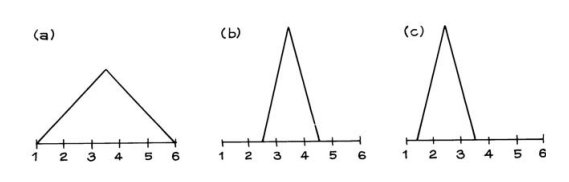
\includegraphics{Figuras/Capítulo 4/4D6.png}
Selecione a alternativa correta. (H(x)=Histograma (x).)
\begin{enumerate}
    \item H(a) - (iv); H(b) - (ii); H(c) - (vi).
    \item H(a) - (i); H(b) - (iii); H(c) - (iv).
    \item H(a) - (vi); H(b) - (iv); H(c) - (iii).
    \item H(a) - (i); H(b) - (ii); H(c) - (v).
    \item H(a) - (iv); H(b) - (i); H(c) - (v).
\end{enumerate}

\textbf{Resposta:(d)Histogramas: (a) - i (b) ii (c) v}

\item (área 1 - desvio padrão) (Hipotético). Em um teste clínico, a coleta de dados geralmente começa na "linha de base", quando
as cobaias são recrutadas para o estudo, mas antes de serem randomizadas para tratamento
ou controle. A coleta de dados continua até o final do acompanhamento. Dois testes clínicos
sobre prevenção de ataques cardíacos, que relatam os dados basais sobre o peso, são mostrados abaixo. 

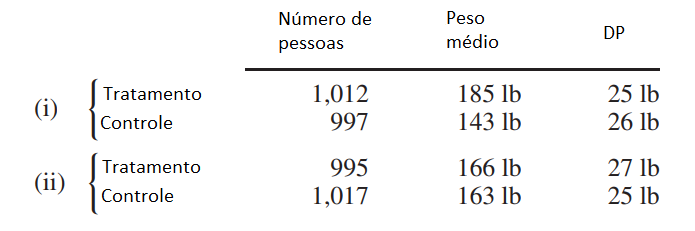
\includegraphics{Figuras/Capítulo 4/4D7.png}

Em um desses testes, a randomização não funcionou. Qual e porquê?

\begin{enumerate}
    \item No teste (i), houve um erro: o grupo de tratamento é muito mais leve que o grupo de controle.
    \item No teste (ii), houve um erro: o grupo de tratamento é muito mais leve que o grupo de controle.
    \item No teste (i), houve um erro: o grupo de tratamento é muito mais pesado que o grupo de controle.
    \item No teste (ii), houve um erro: o grupo de tratamento é muito mais pesado que o grupo de controle.
    \item A diferença de peso médio entre os grupos de tratamento e controle pode ser explicado pela diferença no tamanho da amostra de cada grupo, nos dois testes.
\end{enumerate}

\textbf{Resposta:(c) No teste (i), houve um erro: o grupo de tratamento é muito mais pesado que o
grupo de controle.}

\item (área 1 - amostragem) Um investigador (In1) coleta uma amostra de 100 homens de 18 a 24 anos em uma determinada cidade. Outro (In2)
tira uma amostra de 1.000 desses homens.

Selecione a alternativa incorreta:
\begin{enumerate}
    \item As médias devem ser as mesmas para os dois investigadores.
    \item O desvio-padrão deve ser os mesmo para os dois investigadores.
    \item Os dois investigadores tem a mesma chance de obter o homem mais alto.
    \item In1 é mais provável de obter o homem mais baixo.
    \item A amplitude dos dados deve ser diferente para cada  investigador.
\end{enumerate}

\textbf{Resposta:(c) As médias e os DPs devem ser os mesmos, mas o investigador com a maior amostra é mais provável de obter o homem mais alto e o mais baixo. Maior
a amostra, maior a amplitude. O DP e a amplitude medem coisas diferentes.}

\item (área 1 - desvio padrão)  Os homens da amostra HANES5 tinham uma altura média de 1,75 metros e o DP
era de 8cm. Amanhã, um desses homens será escolhido aleatoriamente. Voce tem que
adivinhar a altura dele. O que você deve adivinhar? Você tem cerca de 1 chance em 3 de estar errado por mais de 
por mais de \_\_\_\_\_\_\_\_. Preencha o espaço em branco.

\begin{enumerate}
    \item 1,25 cm
    \item 8 cm
    \item 13 cm
    \item 2,5 cm
    \item 4 cm
\end{enumerate}

Opções: 1,25cm, 8 cm, 13cm.

\textbf{Resposta:(b) Adivinhe a média, 1,75m. Você tem cerca de 1/3 de uma chance de sair por mais
um DP, que é de 8 cm.}

\item (área 1 - desvio padrão e desvio RMS) Os homens da amostra HANES5 tinham uma altura média de 1,75 metros e o DP
era de 8cm. Amanhã uma série de homens será escolhida aleatoriamente, e você tem que adivinhar a altura deles.
Depois que cada homem aparecer, sua altura real será comparada com o seu palpite para
ver quão longe você estava. A raiz do valor quadrático médio dos erros deve ser \_\_\_\_\_\_\_\_. Preencha o espaço em branco.

\begin{enumerate}
    \item 3,5 cm
    \item 64 cm
    \item 1,25 cm
    \item 8 cm
    \item 13 cm
\end{enumerate}

\textbf{Resposta:(d) 8 cm, o DP é o desvio RMS da média.}
%set E
\item (área 1 - desvio padrão) Adivinhe qual das três listas a seguir tem o maior desvio padrão. E o menor? Verifique seu palpite
calculando o DP para as listas.

(i) 9, 9, 10, 10, 10, 12

(ii) 7, 8, 10, 11, 11, 13

(iii) 15, 13, 14, 14, 14, 14

Quanto ao valor do desvio padrão, é correto afirmar:

\begin{enumerate}
    \item DP(ii) $<$ DP(i) $=$ DP(iii)
    \item DP(iii) $<$ DP(ii) $<$ DP(i)
    \item DP(iii) $<$ DP(i) $<$ DP(ii)
    \item DP(i) $<$ DP(ii) $<$ DP(iii)
    \item DP(ii) $<$ DP(i) $<$ DP(iii)
\end{enumerate}

\textbf{Resposta:(e) O DP de (ii) é o maior e o de (iii) é o menor; de fato, o DP de (i) é 1, o DP de (ii) é 2 e o DP de (iii) é $\approx$ 0.63.}

\item (área 1 - desvio padrão) Duas pessoas estão lhe dizendo como calcular o DP da lista 1, 2, 3, 4, 5:

Pessoa 1 (P1): Como a média é 3, os desvios da média são -2, -1, 0, 1 e 2.
Esqueça os sinais.

O desvio médio é $$\frac{2 + 1 + 0 + 1 + 2}{5}=1,2 $$
e esse é o DP.

Pessoa 2 (P2): Como a média é 3, os desvios da média são -2, -1, 0, 1 e 2.
O 0 não conta, então 

Raiz do valor quadrático médio dos desvios é $$\sqrt{\frac{4 + 1 + 1 + 4}{4}}=1,6 $$
e esse é o DP.

Quem está certo? Ou os dois estão errados? Responda e explique o erro.

\begin{enumerate}
    \item (P1) está certa. (P2) está errada pois o 0 conta.
    \item (P2) está certa. (P1) está errada pois deve ser extraída a raiz quadrada do valor.
    \item Os dois estão errados, (P1) pois o DP é diferente do desvio da média e (P2) pois o 0 conta.
    \item Os dois estão errados, (P1) pois o valor no denominador deve ser n+1 ao invés de n, (P2) pois os valores no numerador não devem ser elevados ao quadrado.
    \item Os dois estão errados, (P1) pois deve ser extraída a raiz quadrada do valor, (P2) pois o denominador também deve ser elevado ao quadrado.
    
\end{enumerate}
\textbf{Resposta:(c)
(P1) Não, o DP é diferente do desvio da média, portanto o método está
errado. (P2) Não, o 0 conta, então o método está errado.
}

\item (área 1 - DP, amplitude) Três instrutores estão comparando as pontuações em suas provas  finais; cada um tinha 99 alunos. Na
classe A, um aluno obteve 1 ponto, outro obteve 99 pontos e o restante obteve 50 pontos.
Na classe B, 49 alunos obtiveram nota 1, um aluno obteve nota 50 e 49 alunos obtiveram 99 pontos. Na classe C, um aluno obteve uma pontuação de 1, um aluno obteve 2, um aluno obteve 3, e assim por diante, até 99.

Selecione a alternativa incorreta:
\begin{enumerate}
    \item Todas as três classes têm a mesma média: 50.
    \item A classe B tem o maior DP; há mais estudantes longe da média.
    \item Todas as três classes têm a mesma amplitude.
    \item A classe C tem o menor DP, há menos estudantes longe da média.
    \item A forma como os dados estão espalhados não é representada somente pela amplitude.
\end{enumerate}

\textbf{Resposta:(d) A classe A tem o menor DP.}

\item (área 1 - média, desvios) Para cada lista abaixo, calcule a média, os desvios da média e o DP.

(i) 1, 3, 4, 5, 7

(ii) 6, 8, 9, 10, 12

Como a lista (ii) está relacionada à lista (i)? Como essa relação é transferida para a
média? Os desvios da média? O DP?

\begin{enumerate}[label=(\Roman*)]

\item A lista (ii) é obtida da lista (i) adicionando 5 a cada entrada. Isso adiciona 5 à
média, mas não afeta os desvios da média. Então, o DP não é afetado.

\item A lista (ii) é obtida da lista (i) adicionando 5 a cada entrada. Isso aumenta a média, aumenta os desvios e o desvio padrão.

\item A média da lista (i) é 4 e o DP é 2.

\item A média da lista (i) é 6 e o DP é 3.

\item A média da lista (i) é 6 e o DP é 4.

\item A média da lista (ii) é 9 e o DP é 5.

\item A média da lista (ii) é 9 e o DP é 2.

\item A média da lista (ii) é 8 e o DP é 4.
\end{enumerate}

Estão corretas as afirmações:

\begin{enumerate}
    \item (I), (IV) e (VII).
    \item (II), (III) e (VI).
    \item (I), (V) e (VIII). 
    \item (I), (III) e (VII).
    \item (II), (IV) e (VI)
\end{enumerate}
Resposta:

(d) (i) média = 4; desvios = −3, −1, 0, 1, 3; DP = 2.

(ii) média = 9; desvios = −3, −1, 0, 1, 3; DP = 2.

 A lista (ii) é obtida da lista (i) adicionando 5 a cada entrada. Isso adiciona 5 a
média, mas não afeta os desvios da média. Então, o DP não é afetado. Adicionar o mesmo número a cada entrada em uma lista não afeta o DP.

\item (área 1 - média, desvios) Para cada lista abaixo, calcule a média, os desvios da média e o DP.

(i) 1, 3, 4, 5, 7

(ii) 3, 9, 12, 15, 21

Como a lista (ii) está relacionada à lista (i)? Como essa relação é transferida para a
média? Os desvios da média? O DP?

\begin{enumerate}[label=(\Roman*)]

\item A lista (ii) é obtida da lista (i) multiplicando cada entrada por 3. Isso multiplica a média por 3, os desvios por 3, mas não interfere no desvio padrão.

\item A lista (ii) é obtida da lista (i) multiplicando cada entrada por 3. Isso multiplica a média por 3, e também os desvios da média por um
fator de 3, o que leva o DP a ser multiplicado por 3.

\item A média da lista (i) é 6 e o DP é 3.

\item A média da lista (i) é 4 e o DP é 2.

\item A média da lista (i) é 3 e o DP é 9.

\item A média da lista (ii) é 12 e o DP é 6.

\item A média da lista (ii) é 10 e o DP é 9.

\item A média da lista (ii) é 12 e o DP é 3.
\end{enumerate}

Estão corretas as afirmações:

\begin{enumerate}
    \item (II), (IV) e (VI).
    \item (II), (III) e (VII).
    \item (I), (V) e (VII). 
    \item (I), (III) e (VIII).
    \item (II), (IV) e (VI)
\end{enumerate}

Resposta:
(a)
(i) média = 4; desvios = −3, −1, 0, 1, 3; DP = 2.

(ii) média = 12; desvios = −9, −3, 0, 3, 9; DP = 6.

A lista (ii) é obtida da lista (i) multiplicando cada entrada por 3. Isso multiplica a média por 3, e também os desvios da média por um
fator de 3, o que leva o DP a ser multiplicado por 3. Multiplicando cada entrada em
uma lista com o mesmo número positivo apenas multiplica o DP por esse número.

\item (área 1 - média, desvios) Para cada lista abaixo, calcule a média, os desvios da média e o DP.

(i) 5, −4, 3, −1, 7

(ii) −5, 4, −3, 1, −7

Como a lista (ii) está relacionada à lista (i)? Como essa relação é transferida para a
média? Os desvios da média? O DP?

\begin{enumerate}[label=(\Roman*)]

\item A lista (ii) é obtida da lista (i) alterando o sinal de cada entrada. Isso
altera a média e de todos os desvios da média, mas não afeta o DP.

\item A lista (ii) é obtida da lista (i) alterando o sinal de cada entrada. Isso
altera a média e todos os desvios da média, o que afeta o DP.

\item A média da lista (i) é 3 e o DP é 5.

\item A média da lista (i) é 2 e o DP é 4.

\item A média da lista (i) é 2 e o DP é 6.

\item A média da lista (ii) é 4 e o DP é 6.

\item A média da lista (ii) é -3 e o DP é 9.

\item A média da lista (ii) é -2 e o DP é 4.
\end{enumerate}

Estão corretas as afirmações:

\begin{enumerate}
    \item (II), (V) e (VII).
    \item (I), (IV) e (VIII).
    \item (I), (V) e (VI). 
    \item (II), (III) e (VII).
    \item (II), (IV) e (VI)
\end{enumerate}

Resposta:

(b)

(i) média = 2; desvios = 3, −6, 1, −3, 5; DP = 4.

(ii) média = -2; desvios = −3, 6, −1, 3, −5; DP = 4.

A lista (ii) é obtida da lista (i) alterando o sinal de cada entrada. Isso
altera o sinal da média e de todos os desvios da média, mas não afeta o DP.

\item (área 1 - influência de uma mudança nos dados na média e no DP)

(I) O governador da Califórnia propõe dar a todos os funcionários estaduais um aumento
de US\$ 250 por mês. De que forma isso afetaria o salário médio mensal dos
funcionários? E o DP?

(II) O que um aumento de 5\% nos salários, em geral, faria com o
salário médio mensal? E com o DP?

As respostas para essas duas perguntas são:

\begin{enumerate}
    \item (I) Aumentaria a média em US\$250, e o DP permaneceria o mesmo.
    (II)Aumentaria a média em 5\%, o DP permaneceria o mesmo.
    \item (I) A média e o DP permaneceriam os mesmos.
    
    (II) Aumentaria o DP em 5\%, a média permaneceria a mesma.
    \item (I) Aumentaria a média e o DP em US\$ 250.
    
    (II) Aumentaria a média em 5\%, e o DP permaneceria o mesmo
    \item (I) Aumentaria o DP em US\$250, mas a média permaneceria a mesma.
    (II)Aumentaria a média em 5\% e o DP em 10\%.
    \item (I) Aumentaria a média em US\$250, e o DP permaneceria o mesmo.
    (II)Aumentaria a média e o DP em 5\%.
\end{enumerate}

\textbf{Resposta: (e)
(I) Isso aumentaria a média em US\$ 250, mas o DP permaneceria o mesmo.
(II) Isso aumentaria a média e o desvio padrão em 5\%.
 }

\item (área 1 - RMS e DP) Qual é a raiz do valor quadrático médio da lista 17, 17, 17, 17, 17? E o DP?

\begin{enumerate}
    \item RMS=0, DP=0.
    \item RMS=17, DP=0.
    \item RMS=0, DP=17.
    \item RMS=17, DP=17.
    \item RMS=4, DP=2.
\end{enumerate}
\textbf{Resposta:(b) A raíz do valor quadrático médio é 17 e o DP é 0.}

\item (área 1 - RMS e DP) Para a lista 107, 98, 93, 101, 104, o que é menor - a raiz do valor quadrático médio ou o DP? Não é necessário fazer as contas.

\begin{enumerate}
    \item São o mesmo valor.
    \item A raiz do valor quadrático médio é muito menor do que o DP.
    \item O DP é muito menor que a raíz do valor quadrático médio.
    \item A raiz do valor quadrático médio é menor do que o DP, mas a diferença é pequena (dif$<$10\%).
    \item O DP é menor do que a raiz do valor quadrático médio, mas a diferença é pequena (dif$<$10\%).
\end{enumerate}

\textbf{Resposta:(c) O DP é muito menor que a raíz do valor quadrático médio.}

\item (área 1 - desvio padrão) (I) O DP pode, em algum caso, ser negativo?

(II) Para uma lista de números positivos, o DP pode, em algum caso, ser maior do que a média?

\begin{enumerate}
    \item (I)Sim. (II)Não.
    \item (I)Não. (II)Não, para isso devem haver números negativos na lista.
    \item (I)Não. (II)Não, não acontece em nenhuma lista, mesmo que houver números negativos.
    \item (I)Sim. (II)Sim.
    \item (I)Não. (II)Sim.
    
\end{enumerate}
\textbf{Resposta:(e)(I) Não.
(II) Sim; por exemplo, a lista 1, 1, 16 tem uma média de 6 e um DP de cerca de 7.}

\end{enumerate}
\end{document}